\chapter{Verwandte Themen}\label{ch:related}
Bloom-Filter sind eine häufig verwendete Datenstruktur und spielen eine wichtige Rolle in AMBIENCE. Somit stellte sich weder die Frage, ob überhaupt Bloom-Filter eingesetzt werden sollen, noch nach ihrer optimalen Implementierung. AMBIENCE diente vielmehr als Schnittstelle für den eigenen Entwurf. 

Dennoch wurden die Bloom-Filter auch selbst implementiert, um die eigenen Berechnungen zu überprüfen und mit realistischen Werten arbeiten zu können. Das folgende Kapitel stellt in Abschnitt \ref{sec:bloom-implementierung} zunächst dar, auf welche Arbeiten und bewährten Techniken dabei Bezug genommen wurde. 

Ziel dieser Arbeit war eine optimale Lösung für das Anwendungsszenario von AMBIENCE. Eine solche wird vom aktuellen Stand der Forschung nicht abgedeckt. Die Darstellung des aktuellen Forschungsstandes konzentriert  sich wegen der Fülle der Einsatzmöglichkeiten auf Bloom-Filter im Zusammenhang mit Netzwerkanwendungen (vgl. \ref{sec:bloom-netzwerk}), Indexstrukturen und die \textit{k}-nächste-Nachbarn-Suche. Überlegungen und Arbeiten, die Eingang in die eigene Implementierung gefunden haben, werden in den Abschnitten \ref{sec:bloom-indexstrukturen} und \ref{sec:bloom-knn} vorgestellt. 
\section{Implementierung von Bloom-Filtern}\label{sec:bloom-implementierung}
Gemäß dem Bloom-Filter-Prinzip bietet sich die Verwendung von Bloom-Filtern an, wenn Speicherplatz effektiv genutzt werden soll und falsch Positive verkraftet werden können (vgl. Abschnitt \ref{sec:bloom-anwendungen}). Die mathematischen Grundlagen wie Minimierung der Falsch-Positiv-Rate, Abschätzung der Anzahl eingefügter Elemente, Abschätzung der Jaccard-Distanz etc. werden von Bloom\footnote{Vgl. \cite{Bloom1970}.}, Broder, Mitzenmacher \footnote{Vgl. \cite{Broder2004} und \cite{Mitzenmacher2002}.} sowie Werner et al.\footnote{Vgl. \cite{Werner2015}.} ausführlich dargestellt, um nur einige zu nennen. 

Wie in den Abschnitten \ref{sec:hashfunktionen} und \ref{sec:bloom-anwendungen} erwähnt, werden Bloom-Filter im Apache-Projekt Cassandra eingesetzt. Sie dienen dort zum schnellen Nachschlagen in Tabellen, den so genannten \textit{SSTables}. Die Cassandra-Entwickler, namentlich Jonathan Ellis, haben sich eingehend mit der Implementierung von Bloom-Filtern und optimalen Hashfunktionen beschäftigt. Diese Überlegungen haben keinen Eingang in wissenschaftliche Veröffentlichungen gefunden, sind jedoch sehr praxisrelevant\footnote{\url{http://cassandra.apache.org/} ist die Hauptseite des Cassandra-Projekts. Der Cassandra-Quellcode ist frei verfügbar unter \url{https://github.com/apache/cassandra}. Datenmodell und Architektur werden z.B. unter \url{http://wiki.apache.org/cassandra/DataModel}, \url{http://wiki.apache.org/cassandra/ArchitectureOverview} und \url{http://prettyprint.me/prettyprint.me/2010/05/02/understanding-cassandra-code-base/index.html} beschrieben. Für diese Arbeit wurden auch eine programmatische Rede (vgl. \url{https://youtu.be/WD1v6jr5fKY}) und ein Blog (vgl. \url{http://spyced.blogspot.de/}) von Ellis berücksichtigt.}. Zur Wahl der Hashfunktionen schreibt Ellis: 
\begin{quote}
[I]t turns out that it's surprisingly hard to find good information on one part of the implementation: how do you generate an indefinite number of hashes? Even small filters will use three or four; a dozen or more is not unheard of\footnote{Vgl. \url{http://spyced.blogspot.de/2009/01/all-you-ever-wanted-to-know-about.html}.}. 
\end{quote}
Die mathematischen Grundlagen für die Generierung von \textit{i} Hashfunktionen mit möglichst gleich verteilten Ergebnissen finden sich bei Kirsch und Mitzenmacher\footnote{Vgl. \cite{Kirsch2006}.}. Viele Bloom-Filter-Implementierungen wie z.B. \textit{PyBloom} verwenden jedoch Hashfunktionen, deren Ergebnisse nicht gleich verteilt sind. Das Problem dabei ist, dass damit häufig eine deutlich höhere Falsch-Positiv-Rate im Bloom-Filter erzielt wird als rechnerisch angenommen. 

Der Grund für die Verwendung minderwertiger Hashfunktionen ist Ellis zu Folge, dass die meisten Implementierungen auf schnelle Berechnung der Hashwerte abzielten statt auf Gleichverteilung der Ergebnisse. Das ist aber für einen Bloom-Filter essentiell, wenn z.B. wie in Cassandra teure Eingabe/Ausgabe-Operationen durch den Einsatz von Bloom-Filtern reduziert werden sollen. Weist der Bloom-Filter eine erhöhte Falsch-Positiv-Rate auf, beispielsweise von 140\% gegenüber dem erwarteten Wert, reduziert das die positiven Effekte des Bloom-Filters drastisch.  

Ellis schlägt zwei Lösungsansätze vor: Entweder kryptografische Hashfunktionen oder Murmur- und Jenkins-Hashfunktionen mit guter Gleichverteilung der Ergebnisse. Kryptografische Hashfunktionen wurden bereits in Abschnitt \ref{sec:hashfunktionen} dargestellt. Der Nachteil daran ist, dass sie in der Regel aufwändiger in der Berechnung sind als gewöhnliche Hashfunktionen. Das spielt z.B. bei der einmaligen Berechnung eines Fingerabdrucks keine große Rolle. Die Performanz von Bloom-Filtern kann dadurch aber beeinträchtigt werden. 

Mit Murmur- oder Jenkins-Hashfunktionen gibt es zwei Möglichkeiten, eine beliebige Anzahl von Hashfunktionen mit guter Gleichverteilung der Ergebnisse zu erzeugen. Entweder berechnet man den \textit{i}-ten Hashwert als $\text{hash0 }+ i\ast \text{hash1}$ wie von Kirsch und Mitzenmacher beschrieben\footnote{Vgl. ebd..} und in Cassandra angewendet. Alternativ nimmt man den \textit{i}-ten Hashwert als Startwert für die Berechnung des \textit{i+1}-ten Hashwerts. Dieser Ansatz wurde in Hadoop gewählt und auch hier verwendet. 

Zur Organisation der Bloom-Filter äußert sich Ellis ebenfalls, jedoch nur auf seinem Twitter-Account und ohne auf Details einzugehen: 
\begin{quote}
Rather than naively checking every Bloom Filter for the element, organize the BF in a hierarchy akin to B+ tree\footnote{Vgl. \url{https://twitter.com/spyced/status/707266703751651328}.}.
\end{quote}
Zwar ist hier offensichtlich von der Suche nach einem Element in einem Bloom-Filter die Rede, nicht nach einem Bloom-Filter selbst wie in AMBIENCE. Dennoch zeichnet sich ab, dass ein B$^+$-Baums als Indexstruktur für Bloom-Filter in Erwägung gezogen werden sollte. 

Damit sind die Gemeinsamkeiten zwischen Cassandra und AMBIENCE erschöpft. Es war zunächst überlegt worden, Cassandra zur Evaluation der eigenen Implementierung zu nutzen, d.h. die eigenen Datensätze in eine lokale Cassandra-Installation zu überführen und z.B. die Laufzeiten der \textit{k}-nächste-Nachbarn-Suche zu vergleichen. Der entscheidende Unterschied zur Verwendung der Bloom-Filter in Cassandra ist jedoch, dass in AMBIENCE die Bloom-Filter selbst die Datensätze sind, während sie in Cassandra zum Nachschlagen der Datensätze verwendet werden. Damit erwies sich die Evaluation mit Cassandra als nicht praktikabel. Die Publikationen aus dem Cassandra-Umfeld wurden daher ausschließlich bezüglich Implementierung der Bloom-Filter, Wahl und Berechnung der Hashfunktionen berücksichtigt. Der Hinweis auf B$^+$-Bäume in Zusammenhang mit Bloom-Filtern unterstützte zudem die Entscheidung für diese Indexstruktur. 
\section{Netzwerkanwendungen mit Bloom-Filtern}\label{sec:bloom-netzwerk}
Bloom-Filter werden in zahlreichen Netzwerk-Anwendungen eingesetzt. Das erscheint auf den ersten Blick interessant für AMBIENCE als soziales Online-Netz. Ein guter Überblick über Netzwerk-Anwendungen mit Bloom-Filtern findet sich bei Broder und Mitzenmacher:  
\begin{quote}
The aim of this paper is to survey the ways in which Bloom filters have been used and modified in a variety of network problems, with the aim of providing a unified mathematical and practical framework for understanding them and stimulating their use in future applications\footnote{\cite{Broder2004}: 485.}.
\end{quote}
Die Autoren beschreiben unter anderem die Verwendung von Bloom-Filtern zur Kollaboration in Overlay- und Peer-to-Peer-Netzwerken\footnote{Vgl. ebd.: 486.}. Jedoch besteht ein entscheidender Unterschied zur Fragestellung. Zwar werden die Anfragen von einem mobilen Endgerät an einen Host gesendet, also über das Netzwerk übertragen. Die der \textit{k}-nächste-Nachbarn-Suche bezieht sich jedoch auf die Menge der an einem Host gespeicherten Bloom-Filter. Unter diesen sollen die ähnlichsten möglichst schnell und effizient gefunden werden, aber ab diesem Zeitpunkt werden keine Nachrichten mehr im Netzwerk übertragen. Die \textit{k}-Nächste-Nachbarn-Suche findet vielmehr auf einem Host statt und erst das Ergebnis wird an das anfragende Gerät übermittelt. 

Ähnlich verhält es sich bezüglich der Arbeit von Agarwal und Trachtenberg. Darin werden Counting Bloom-Filter verwendet, um die Abschätzung von Mengendifferenzen auf unterschiedlichen Hosts zu optimieren \footnote{Vgl. \cite{Agarwal2006}.}. Daran werden zwar die Vorteile von Bloom-Filtern bei der blinden Kalkulation von Mengenunterschieden deutlich, ohne dass ihre Elemente bzw. die Objekte in den Bloom-Filtern bekannt sein müssen. Wie bei Werner et al. beschrieben, kann diese Eigenschaft den Schutz der Privatsphäre in einem sozialen Online-Netz verbessern\footnote{Vgl. \cite{Werner2015}: 2 und 5.}. Auch hier findet die Abschätzung der Mengendifferenzen jedoch zwischen zwei unterschiedlichen Hosts statt, weswegen dieser Ansatz für AMBIENCE nicht genutzt werden kann. Gleiches gilt für die Arbeiten von Byers et al.\footnote{Vgl. \cite{Byers2002}.}, Shiraki et al.\footnote{Vgl. \cite{Shiraki2009}}, Zhang\footnote{Vgl. \cite{Zhang2012}.} und Zhu et al.\footnote{Vgl. \cite{Zhu2004}.}. In all diesen Arbeiten werden Bloom-Filter im Zusammenhang mit Netzwerken eingesetzt. Das spezifische Szenario von AMBIENCE wird jedoch von keiner dieser Arbeiten abgedeckt. 
\subsection{Indexstrukturen für Bloom-Filter}
Ein Überblick über Indexstrukturen für Datenbank-Managementsysteme auf Hauptspeicherbasis findet sich bei Lehman und Carey\footnote{Vgl. \cite{Lehman1896}.} Die Publikation zählt nicht zu den Neuesten, kann aber zu einem besseren Verständnis der Indexstrukturen aus Abschnitt \ref{sec:indexstrukturen} beitragen. Wichtig ist vor allem die Erkenntnis, dass der Einsatz einer Hauptspeicher-Datenstruktur sinnvoll ist, wenn um die Performanz von Anfragen auf größeren Datenmengen zu verbessern. B- und B$^+$-Bäume werden allgemein als Hauptspeicher-Datenstruk\-turen verwendet, d.h. ein Vorteil ist die Reduzierung der Plattenzugriffe bei der Suche nach Datensätzen. In der Regel benötigen sie viel weniger Speicherplatz als das tatsächliche Datenaufkommen. Unter anderem kann mit Zeigern gearbeitet werden, ohne alle vorhandenden Daten physisch in der Datenstruktur halten zu müssen. 

Nachdem klar war, dass die Organisation der Bloom-Filter durch eine geeignete Indexstruktur erfolgen könnte, wurde mit der Suche begonnen. Adaptierungen der kanonischen Formen für spezifische Anwendungen finden sich in der Literatur zu Hauf. Wenig überraschend ist keine darunter, die das spezifische Szenario von AMBIENCE abbildet.

Hellerstein und Pfeffers\footnote{Vgl. \cite{Hellerstein1994}.} Publikation von 1994 stellt den \textit{RD-Tree} als Indexstruktur für objektrelationale Geo-Datenbanken vor. Abgesehen davon, dass der objektrelationale Ansatz mittlerweile kaum noch verfolgt wird, ist die Anwendung für Geodaten vorgesehen. Diese haben spezielle Eigenschaften wie z.B. Inklusionsbeziehungen zwischen Punkten und Flächen oder Flächen untereinander. Diese Eigenschaften müssen in der Indexstruktur abgebildet werden und von Suchanfragen unterstützt werden. Indexstrukturen für Geodaten erschienen daher für die Fragestellung ungeeignet, da sie einerseits einen unnötigen Implementierungsaufwand erfordern, der für die vorhandenen Daten nicht erforderlich wäre, andererseits die \textit{k}-Nächste-Nachbarn-Suche unnötig erschweren. Zu diesen Indexstrukturen zählt auch der \textit{R-Baum}, der der Organisation von minimalen umgebenden Rechtecken dient. Eine Abwandlung hiervon präsentiert die Arbeit von Yang und Lin, die als neue Indexstruktur den \textit{bichromatic Rdnn-Tree} vorstellen\footnote{Vgl. \cite{Yang2002}}. Diese Arbeit erschien insofern von Interesse, als die Autoren nicht nur Punkt-Anfragen, sondern \textit{k-}Nächste-Paare und \textit{k}-Nächste-Nachbarn-Paare betrachten und ihre Indexstruktur dafür optimiert haben. Mangels Ähnlichkeit von Bloom-Filtern und spatialen Datensätzen musste auch dieser Ansatz verworfen werden. 

Am stärksten wurde schließlich die Arbeit "`Evaluation of the Structured Bloom Filters Based on Similarity"' von Hiroshi Sakuma und Fumiaki Sato berücksichtigt\footnote{Vgl. \cite{Sakuma2011}.}. Die Autoren behandeln zwar ein Netzwerk-Problem, doch ließen sich Teile der Indexstruktur für AMBIENCE adaptieren. Kern der Arbeit ist ein Baum aus Bloom-Filtern zur Minimierung der Weiterleitungen von Anfragen in einem Verteilten System. 
\begin{figure}[hpbt]
  \centering
  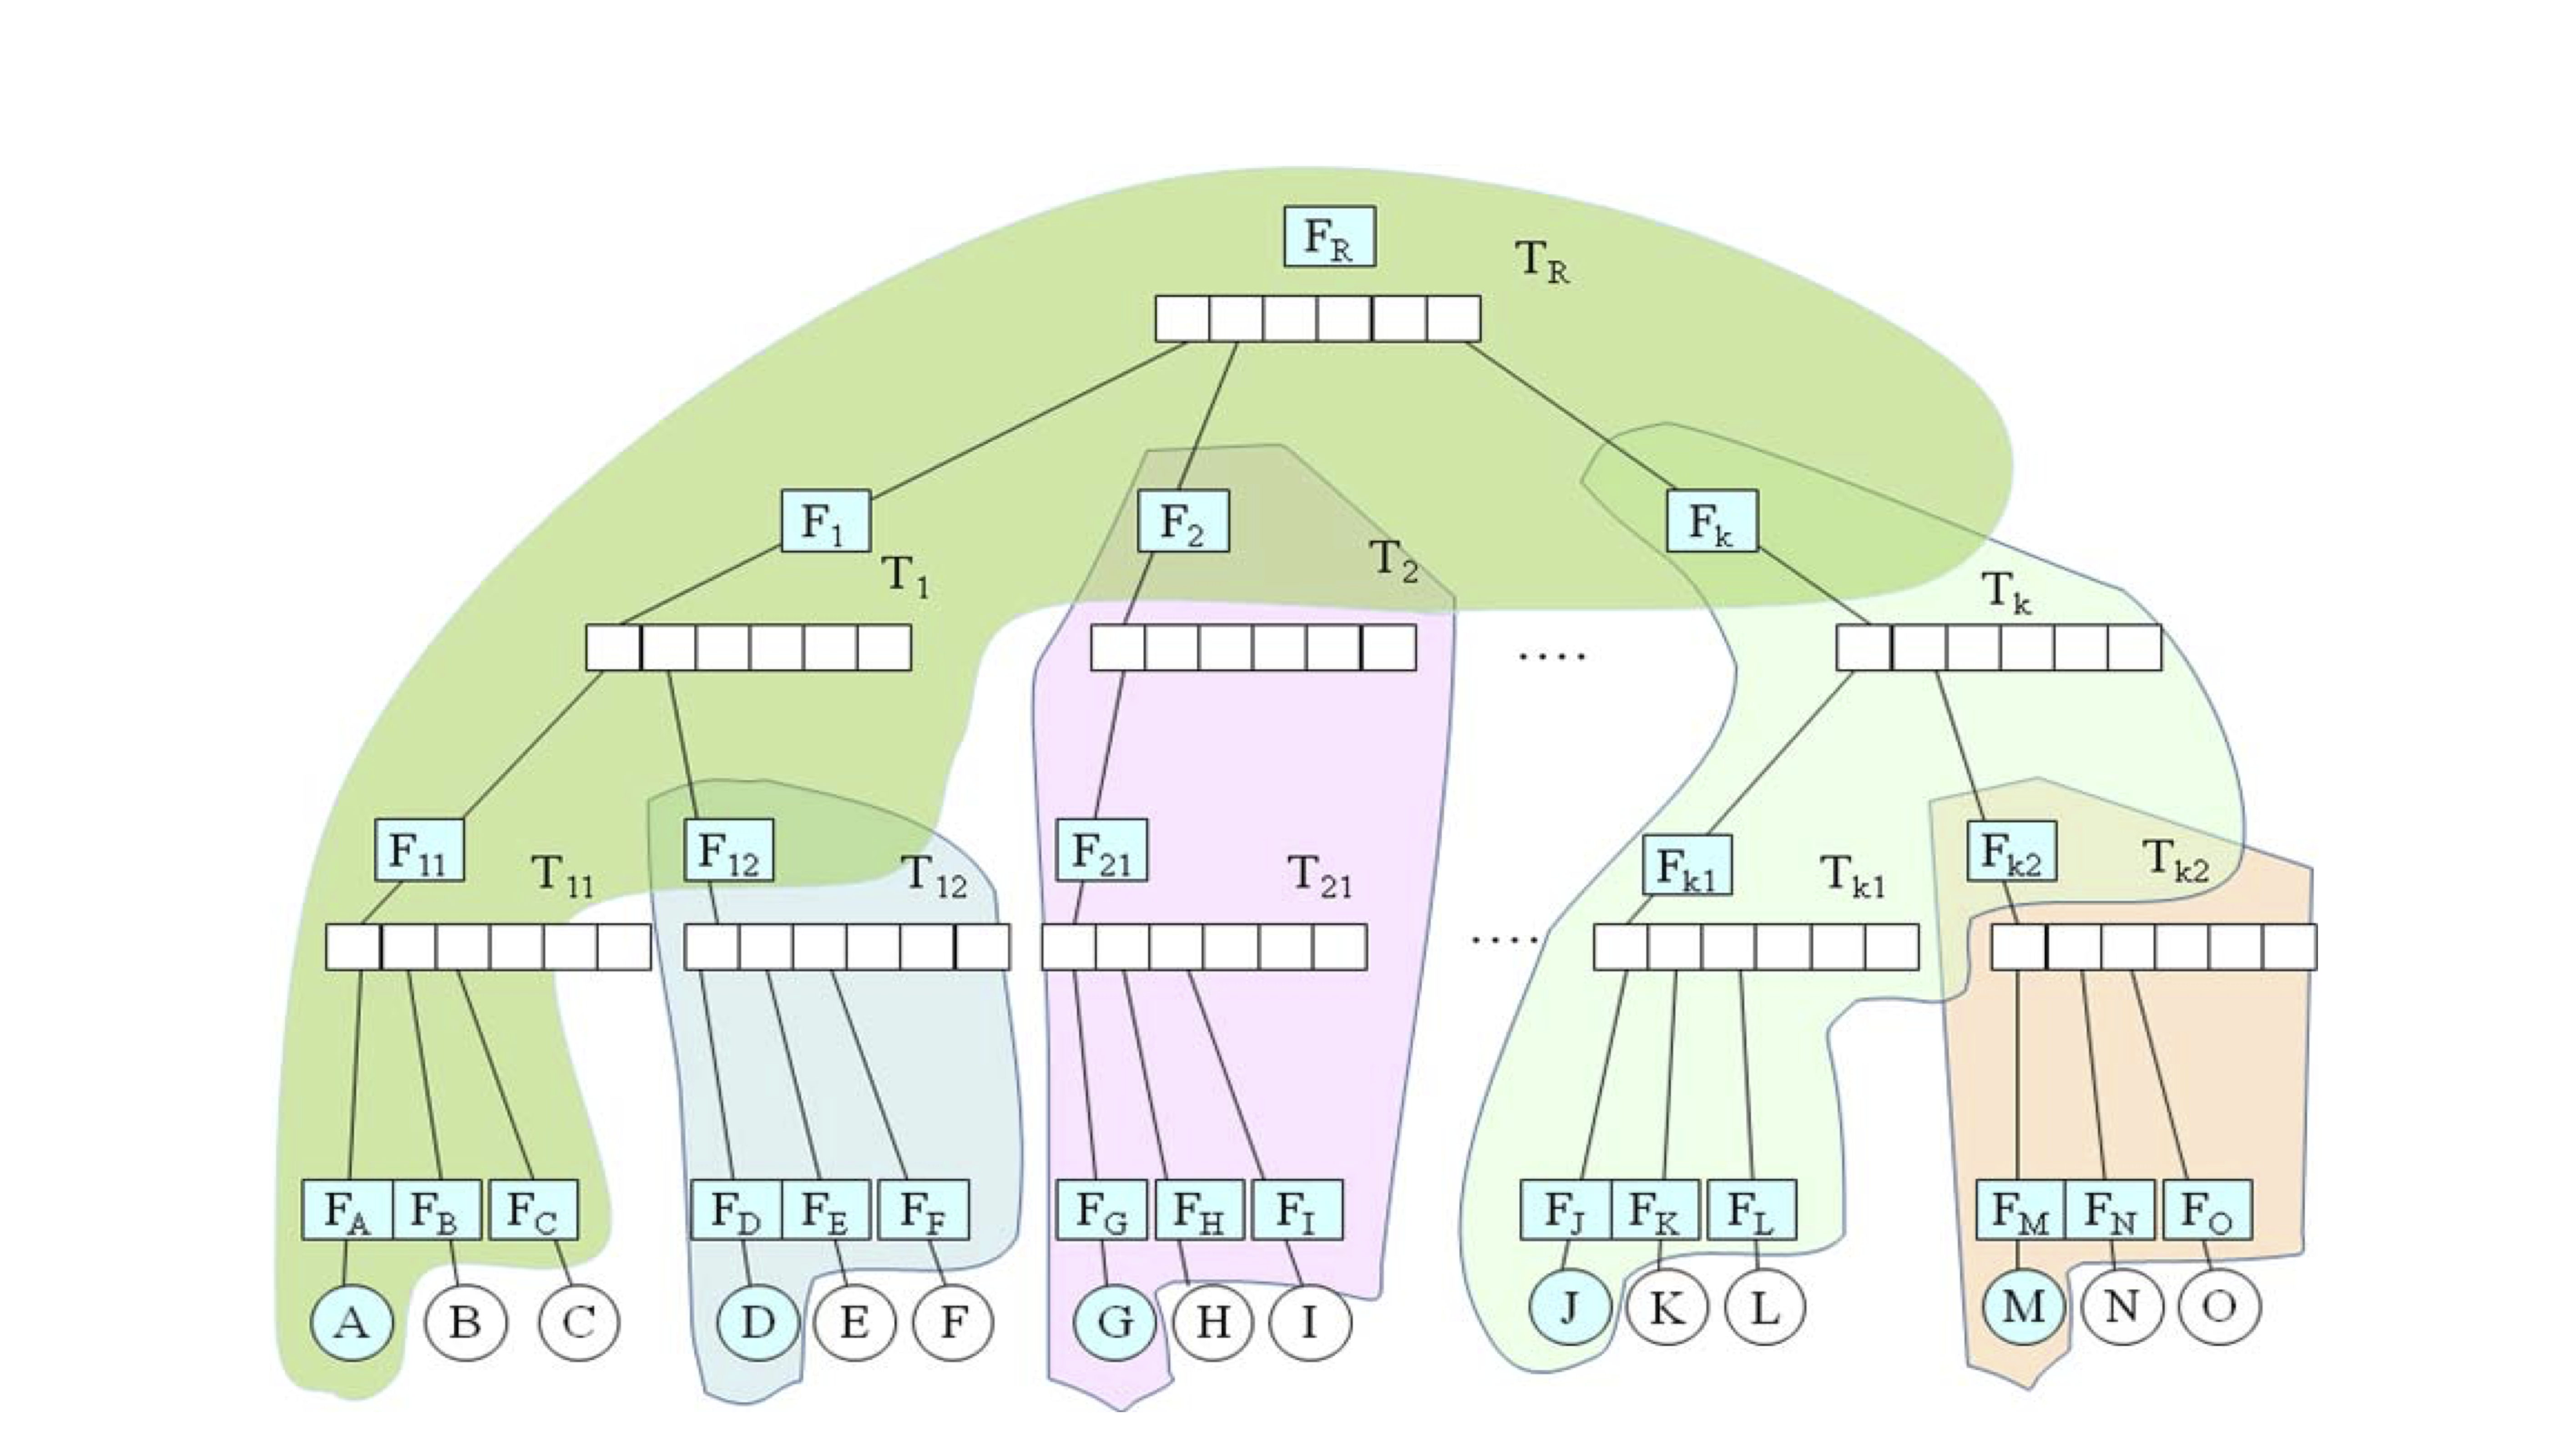
\includegraphics[width=1.0\textwidth]{pictures/bloom-filter-baum.png}\\
  \caption[Bloom-Filter-Baum bei Sakuma und Sato (Bildnachweis: \cite{Sakuma2011}: 320)]{Bloom-Filter-Baum bei Sakuma und Sato (\cite{Sakuma2011}: 320).}\label{fig:pic5}
\end{figure}
Die Indexstruktur ist ein Baum aus Bloom-Filtern, an dem jeder im Netzwerk beteiligte Knoten einen Teil hält (vgl. Abb. \ref{fig:pic5}). Er ist nach Ähnlichkeit zwischen Bloom-Filtern aufgebaut. Wie in Abschnitt \ref{sec:distanzmasse} beschrieben, dient als Ähnlichkeitsmaß jedoch nicht die Jaccard-Distanz, sondern die Anzahl gleicher 1-Bits. Die Datensätze werden nicht im Baum selbst gehalten, sondern die Knoten des Baums dienen dem Management bzw. der Organisation. Da es sich um ein Verteiltes System handelt, aus dem Knoten ausscheiden oder neu hinzukommen können, müssen regelmäßige Updates per Broadcast-Nachrichten an alle Knoten im Baum propagiert werden. Ein Knoten ist darin für den unter ihm liegenden Teilbaum verantwortlich. D.h. in Abb. \ref{fig:pic5} hält der Wurzelknoten hält Informationen über das gesamte Netzwerk, Knoten \textit{F2} hält Informationen über den violetten Teilbaum. 

Die Autoren gehen besonders auf zwei Operationen ein, die on ihnen evaluiert und mit bestehenden Methoden verglichen werden: Anzahl der Schritte bei der Anfrage-Weiterleitung und Restrukturierung des Baumes beim Ausscheiden und Hinzufügen von Knoten\footnote{Vgl. ebd.: 316.}. Die Anfrage-Weiterleitung basiert dabei auf der Baumstruktur, die Restrukturierung auf der Anordnung der Bloom-Filter nach Ähnlichkeit. Beide Aspekte sind für AMBIENCE weniger relevant: Erstens findet die k-Nächste-Nachbarn-Suche auf ein und demselben Host statt. Anfragen müssen also nicht an andere Hosts weiter geleitet werden. Daher wurde darauf verzichtet, in inneren Knoten Informationen über die Geschwisterknoten vorzuhalten. 

% \cite{Jannink1995} (Löschen im B+-Tree) 
% Sakuma 

\section{\textit{k}-nächste-Nachbarn-Suche}\label{sec:bloom-knn}

% Bayardo 
